%#######################################
% Original: Oktober.2011; Prof. Dr. Martin Grüttmüller, FIM
% Last Edit: Dezember.2021; M.Eng. Mario Hoffmann, Fakultät DIT
% Reimport: April.2022; Prof. Dr. Jean-Alexander Müller, Fakultät Informatik und Medien
%#######################################

%!TEX TS-program = lualatex
%!TEX encoding = UTF-8 Unicode
%!TEX root = Bachelorarbeit.tex
%!TEX spellcheck = de_DE
%!BIB program = biber

\documentclass[
    a4paper,
    12pt,
    numbers=noenddot,
    parskip,
    toc=flat,
    toc=listof,
    toc=bibliography,
    twoside=false,
    captions=tableheading]{scrbook}


%##########################################################
% Einbinden aller Pakete etc.
%##########################################################

%!TeX root = ./../Bachelorarbeit.tex

%##########################################################
% Dokumentenangaben
%##########################################################

% ---- Studiengang ----
\newcommand{\studiengang}{Informatik}
\newcommand{\studienganggrad}{Bachelor of Science}
\newcommand{\fakultaet}{Informatik und Medien}
\newcommand{\hochschule}{Hochschule für Technik, Wirtschaft und Kultur}

% ---- Autor + Gutachter ----
\newcommand{\autor}{Jonas Schulze}
\newcommand{\geburtsort}{Hohenmölsen}
\newcommand{\geburtstag}{23.04.2001}

\newcommand{\erstgutachter}{Prof. Dr.-Ing. Jean-Alexander Müller}
\newcommand{\instituteErstgutachter}{HTWK Leipzig}
\newcommand{\zweitgutachter}{M. Sc. Robin Escherich}
\newcommand{\instituteZweitgutachter}{SENEC GmbH}

% ---- Titel, etc ----
\newcommand{\abschlussarbeit}{Bachelorarbeit}
\newcommand{\titel}{Emulation eines 32 Bit Mikrocontrollers zur virtualisierten Ausführung einer Embedded Software Applikation}
% Falls kein Untertitel, einfach leer lassen
\newcommand{\subtitel}{}
\newcommand{\ort}{Leipzig}

% ---- Betreuender Betrieb ----
\newcommand{\betrieb}{SENEC GmbH}

%!TeX root = ./../Bachelorarbeit.tex


%##########################################################
% Pakete - Stil, Sprache und Schriftart
%##########################################################
\usepackage[UKenglish,ngerman]{babel}
\usepackage[T1]{fontenc}
\usepackage[osf,scale=1.15]{sourcesanspro}
\usepackage{csquotes}
\usepackage[headsepline]{scrlayer-scrpage}
\usepackage{fontspec}
\setcounter{tocdepth}{\subsubsectiontocdepth}
\addtokomafont{chapterentry}{\bfseries}
\usepackage[onehalfspacing]{setspace}
%## #### #### ####### ###
\usepackage[absolute, overlay]{textpos}
\usepackage{svg}

% Bib Literatur Verweise
\usepackage[
	backend=biber,
	style=numeric,
	bibencoding=utf8]{biblatex}
\addbibresource{Literatur.bib}

\AtBeginDocument{%
	\providecaptionname{ngerman}{\lstlistlistingname}{Quellcodeverzeichnis}
	\providecaptionname{ngerman}{\lstlistingname}{Quellcode}
}

%##########################################################
% Pakete - Grafisches Elemente und Farben
%##########################################################
\usepackage{graphicx}
\usepackage{xcolor}

\providecommand{\keywords}[1]{\textbf{\textit{Keywords:}} #1}

%############ HTWK Farben #################
\xdefinecolor{htwkGelb}{rgb}{0.996,0.925,0}
\xdefinecolor{htwkGrau}{rgb}{0.945,0.945,0.945}
\xdefinecolor{htwkBlau}{rgb}{0,0.273,0.597}
\xdefinecolor{htwkMagenta}{rgb}{0.894,0,0.488}
\xdefinecolor{htwkRot}{rgb}{0.894,0.1875,0.035}
\xdefinecolor{htwkGruen}{rgb}{0,0.586,0.304}
\xdefinecolor{htwkCyan}{rgb}{0,0.617,0.886}
\xdefinecolor{codegreen}{rgb}{0,0.6,0}
%######## Legen Sie die Farbe fest #####
% htwkBlau, htwkGruen, htwkRot, htwkCyan, htwkGelb, htwkMagenta, htwkGrau
\newcommand{\farbe}{htwkBlau}
\newcommand{\urlfarbe}{htwkBlau}
\newcommand{\citefarbe}{htwkBlau}
%#########################################

% Linkformatierung
\usepackage[
	    colorlinks=true,
	    urlcolor={\urlfarbe},
	    citecolor={\citefarbe},
		pdftitle={\titel},
		pdfauthor={\autor},
		breaklinks=true,
		hidelinks
]{hyperref}

%##########################################################
% Pakete - Zusätzliche
%##########################################################

\usepackage{listings}
\usepackage{scrhack}
\usepackage{microtype}
\usepackage{acro}
% Used for subfigure command
\usepackage{subcaption}

%##########################################################
% Code Snippet Definitionen
%##########################################################
\newcommand\digitstyle{\color{black}}
\makeatletter
\newcommand{\ProcessDigit}[1]
{%
  \ifnum\lst@mode=\lst@Pmode\relax%
   {\digitstyle #1}%
  \else
    #1%
  \fi
}

\lstdefinestyle{MyStyle}{
	basicstyle=\footnotesize\sffamily,
	keywordstyle=\color{blue},
	commentstyle=\color{codegreen},
	stringstyle=\color{orange!80!black},
	morecomment=[l]{//},
	morecomment=[l]{/*}{*/},
	morestring=[b]",
	morestring=[b]',
	breakatwhitespace=false,
    breaklines=true,
    keepspaces=true,
	showspaces=false,
    showstringspaces=false,
    showtabs=false,
    tabsize=2,
	numbers=left,
	numberstyle=\tiny,
	frameround=tttt,
	frame=trbl,
	columns=fullflexible,
	xleftmargin=0.03\linewidth,
	xrightmargin=0.01\linewidth,
	inputencoding=utf8,
}

\lstset{
	style=MyStyle,
	literate=%
    {0}{{{\ProcessDigit{0}}}}1
    {1}{{{\ProcessDigit{1}}}}1
    {2}{{{\ProcessDigit{2}}}}1
    {3}{{{\ProcessDigit{3}}}}1
    {4}{{{\ProcessDigit{4}}}}1
    {5}{{{\ProcessDigit{5}}}}1
    {6}{{{\ProcessDigit{6}}}}1
    {7}{{{\ProcessDigit{7}}}}1
    {8}{{{\ProcessDigit{8}}}}1
    {9}{{{\ProcessDigit{9}}}}1
}

%!TeX root = ./../Bachelorarbeit.tex

%##########################################################
% Inhalt
%##########################################################

\DeclareAcronym{htwk}{
    short = HTWK,
    long = Hochschule für Technik{,} Wirtschaft und Kultur Leipzig
}

\DeclareAcronym{fim}{
    short = FIM,
    long = Fakultät Informatik und Medien
}

\DeclareAcronym{can}{
    short = CAN,
    long = Controller Area Network
}

\DeclareAcronym{ram}{
    short = RAM,
    long = Random Access Memory
}

\DeclareAcronym{arm}{
    short = ARM,
    long = Advanced RISC Machines
}

\DeclareAcronym{cpu}{
    short = CPU,
    long = Central Processing Unit
}

\DeclareAcronym{jtag}{
    short = JTAG,
    long = Joint Test Action Group
}


%##########################################################
% Begin des Dokumentes
%##########################################################
\begin{document}

%!TeX root = ./../Bachelorarbeit.tex

\pagestyle{scrheadings}
\clearpairofpagestyles

\ofoot[\pagemark]{\pagemark}
\ohead{\headmark}
\automark{chapter}

%!TeX root = ./../Bachelorarbeit.tex

%##########################################################
% Titelseite
%##########################################################

\begin{titlepage}
	\noindent
\begin{textblock*}{4.74cm}(16.7mm,11mm)

\includegraphics[width=4.74cm]{anlagen/bilder/logos/HTWK-Fakultaetszusatz_IM_schwarz_de-eps-converted-to.pdf}
\end{textblock*}
\begin{center}

\vspace*{0.5cm}

\large
{\textsc{\Large \abschlussarbeit}}

\vspace*{0.5cm}
zur Erlangung des akademischen Grades\\[0.6cm]
\studienganggrad\\[0.6cm]
im Studiengang \studiengang\\
der Fakultät \fakultaet\\
der \hochschule\ \ort\\

{\LARGE \textbf{\titel}}\\
{\LARGE \textbf{\subtitel}}

\end{center}

%##########################################################
% Autor/in
%##########################################################

\vspace*{2cm}
vorgelegt von: \autor\\
Geburtsort: \geburtsort\\
Geburtsdatum: \geburtstag\\
Abgabe: \ort, den \today


\vspace*{1cm}
\large
\begin{tabbing}
\hspace{4cm}\=\kill
Erstgutachter:  \> \erstgutachter, \instituteErstgutachter\\ 
Zweitgutachter: \> \zweitgutachter, \instituteZweitgutachter\\
\end{tabbing} 

\begin{textblock*}{8.41cm}(18mm,268.3mm)

\includegraphics[width=8.41cm]{anlagen/bilder/logos/htwk-logo-eps-converted-to.pdf}
\end{textblock*}

\end{titlepage}


%##########################################################
% Sperrvermerk
% Ist vorher abzuklären!
%##########################################################
\pagenumbering{gobble}
%%!TeX root = ./../MusterAbschlussarbeit.tex

%##########################################################
% Inhalt
%##########################################################

\thispagestyle{empty} % no page number
\chapter*{Sperrvermerk}

\noindent
Die vorliegende Bachelorarbeit mit dem Titel \titel{} beinhaltet interne vertrauliche Informationen der Firma \betrieb{} des Autors oder patentrechtlich relevante Informationen. 

Die Weitergabe des gesperrten Inhaltes der Arbeit und eventuell beiliegender
Zeichnungen und Daten im Gesamten oder in Teilen ist grundsätzlich untersagt. Es dürfen keinerlei Kopien oder
Abschriften -- auch in digitaler Form -- gefertigt werden. 
Ausnahmen bedürfen der vorherigen schriftlichen Genehmigung der Firma \betrieb{} oder des Autors.

%Hier kommen die Unterschriften hin
\vspace{1.5cm}
\begin{tabular}{p{7cm}p{.5cm}p{7cm}}
	\dotfill & & \dotfill \\\\
	Ort, Datum, Unterschrift \erstgutachter & & Ort, Datum, Unterschrift \zweitgutachter \\
    & & \\\\
    & & \\\\
    \dotfill \\\\
    Ort, Datum, Unterschrift \autor
\end{tabular}


%##########################################################
% Eidesstaatliche Erklärung
%##########################################################
%!TeX root = ./../Bachelorarbeit.tex

%##########################################################
% Inhalt
%##########################################################

\clearpage
\thispagestyle{empty}
\chapter*{Eidesstattliche Erklärung}

Hiermit erkläre ich, dass ich die an der Hochschule für Technik, Wirtschaft und Kultur Leipzig, konkret an der \ac{fim}, eingereichte Arbeit zum Thema \titel{} selbstständig, ohne Hilfe Dritter und ohne Benutzung anderer als der angegebenen Quellen und Hilfsmittel verfasst habe. 

Alle den benutzten Quellen wörtlich oder sinngemäß entnommenen Stellen sind als solche einzeln kenntlich gemacht. Die Abbildungen in dieser Arbeit wurden von mir selbst erstellt oder mit einem entsprechenden Hinweis auf die Quelle versehen.

Diese Arbeit ist bislang keiner anderen Prüfungsbehörde vorgelegt und auch nicht veröffentlicht worden.

Ich bin mir bewusst, dass eine falsche Erklärung rechtliche Folgen haben wird.

\noindent

\vspace{3cm}
\begin{tabular}{p{7cm}p{.5cm}}
    \dotfill \\\\
    Unterschrift \autor\\
    \ort, den \today
\end{tabular}


%##########################################################
% Vorwort (optional)
%##########################################################
%!TeX root = ./../MusterAbschlussarbeit.tex

%##########################################################
% Inhalt
%##########################################################
\clearpage
\chapter*{Vorwort (optional)}
In einem Vorwort können persönliche Danksagungen, Ihre eigene Motivation sowie persönliche Erkenntnisse niederschreiben. 
Inhaltliche Angaben zum Werk werden jedoch nicht gemacht. Zudem ist es möglich hier eine Gendererklärung abzugeben.
Gendererklärung:
In dieser Arbeit wird aus Gründen der besseren Lesbarkeit das generische Maskulinum verwendet. 
Weibliche und anderweitige Geschlechteridentitäten werden dabei ausdrücklich mitgemeint, soweit es für die Aussage erforderlich ist.


%##########################################################
% Abstract/Kurzfassung
%##########################################################
%!TeX root = ./../Bachelorarbeit.tex

%##########################################################
% Inhalt
%##########################################################

\clearpage
\chapter*{Kurzfassung}

Steigende Anforderungen an die Entwicklung von Embedded Software machen
effiziente Entwicklungsprozesse und gute Werkzeuge immer wichtiger.
Die Emulation von Mikrocontrollern kann helfen den manuellen Testaufwand zu
reduzieren und mehr Zeit für Entwicklung zu schaffen.

QEMU ist eine Anwendung zur Emulation verschiedener Hardware Architekturen.
In dieser Arbeit werden zwei verschiedene Ansätze für die Emulation des
STM32F429 Mikrocontrollers untersucht.

Der erste Ansatz beschäftigt sich mit der Erweiterung des bestehenden QEMU
Projekts durch den neuen STM32F429-SoC.
Das Gerät soll bestehende, kompatible Peripherien einbinden und durch eine neue
Implementation des GPIO Controllers erweitert werden.
Anschließend sollen Embeded Software Applikation die Korrektheit der
Implementation testen.
Der zweite Ansatz beschäftigt sich mit der Erweiterung QEMUs durch 
Möglichkeiten der Interprozesskommunikation.
Das \enquote{External Device Interface} wird prototypisch implementiert, auf
den STM32F429 angepasst und in QEMU getestet.

Die Emulation mittels QEMU erweist sich als vielversprechend.
Dennoch sind Implementationsaufwand und Komplexität hoch.
Konfigurationsfehler und eine unvollständige Peripherie Abdeckung kosten Zeit
bei der Fehlersuche, unabhängig vom gewählten Ansatz.
Der Fokus muss vorerst auf einer Vervollständigung der Emulation liegen.
Alternative Möglichkeiten zur Nutzung, wie automatische Tests, sollten
ebenfalls betrachtet werden.

\keywords{QEMU, Embedded Software, Emulation, Mikrocontroller, Programmierung}


%##########################################################
% Inhaltsverzeichnis
%##########################################################
\tableofcontents

%##########################################################
% Abbildungsverzeichnis
%##########################################################
\listoffigures

%##########################################################
% Tabellenverzeichnis
%##########################################################\
\listoftables

%##########################################################
% Quelltextverzeichnis
%##########################################################\
\lstlistoflistings
\clearpage

%##########################################################
% Abkürzungsverzeichnis
%##########################################################
\printacronyms[name=Abkürzungsverzeichnis, heading=chapter*]
\addcontentsline{toc}{chapter}{Abkürzungsverzeichnis}

%##########################################################
% Erstes Kapitel
%##########################################################
%!TeX root = ./../Bachelorarbeit.tex

%##########################################################
% Inhalt
%##########################################################
\pagenumbering{arabic}
\chapter{Einleitung}

Der Leser Ihrer Arbeit sollte die Einleitung (auch als \enquote{Hintergrund} oder \enquote{Problemstellung} bezeichnet) als eine Art Rundblick erleben, 
der die Landschaft darstellt, mit der der Autor konfrontiert wurde, als die Arbeit entstand. Wann und wie hat sich dieses Forschungsthema erstmals angeboten? 
Was hat deutlich gemacht, dass es interessante Fragen gibt, die beantwortet werden müssen? Welche Handlungen und Zusammenhänge waren damals schon erkennbar, und welche Schlüsselinformationen fehlten? 

In der Regel wird in der Einleitung auch ein methodischer Ansatz zur Lösung des Problems vorgeschlagen, 
der möglicherweise durch konkrete Beispiele für die Anwendung dieses Ansatzes unter anderen Umständen veranschaulicht wird. 
Achten Sie beim Schreiben darauf, dass Sie klar zwischen Ihrer Arbeit und anderen Beiträgen unterscheiden müssen.

Bei umfangreichem Material, das Sie hier behandeln möchten, könnte es sich lohnen, die Einleitung in Unterabschnitte zu unterteilen.

Kein anderer Abschnitt in der Arbeit hängt so sehr von der Literaturrecherche ab wie die Einleitung \cite{aoscw2004}. 
Bevor Sie mit der Arbeit an Ihrem Projekt begonnen haben, haben Sie sicher einige wichtige Hintergrundartikel gelesen, 
die Ihnen Ihr Betreuer schon empfohlen hat, aber Sie haben sie wahrscheinlich in letzter Zeit nicht mehr gelesen. 
Jetzt müssen Sie diese nicht nur erneut lesen, sondern sich auch eingehend mit den darin enthaltenen Verweisen befassen, 
um sich mit allen wichtigen Informationsquellen vertraut zu machen. Dies wird Sie natürlich auch in die Lage versetzen, 
frühere Arbeiten kritisch zu bewerten.

\newpage

\section{Ein Beispielabschnitt mit diversen Dingen und Erläuterungen}
Zunächst ein Beispiel für Tabellen. Wichtig ist, dass die Tabellenbeschriftung a) da ist und b) \underline{über} der Tabelle steht. Die Lesenden wollen wissen was sie sehen, bevor sie in die Tabelle eintauchen.
Die hier gezeigte Tabelle ist ohne zusätzliche Pakete verwendbar. Alternativ wäre \texttt{longtable} einzubinden und zu verwenden.

\begin{table}[!h]
    \caption[Tabellenbeschriftung]{Tabellenbeschriftung \cite{Tane2014}}
    \centering
    \begin{tabular}{|c|c|c|}
        \hline
        ID & Kapitel & Seiten \\\hline
        0 & 1 & 5 \\\hline
    \end{tabular}
    \label{tab:Beispieltabelle}
\end{table}

Darüber hinaus drei Beispiele für Programm-Code. Im Ordner \glqq Programmcode\grqq{} sind drei Beispiele für C-, Python- und \ac{html}-Code, welche nachfolgend eingebunden ist.
Es empfiehlt sich ganze Dateien einzubinden, statt den Quellcode hier abzutippen.\\
Der Style ist fest definiert und muss nicht abgeändert werden. In aller Regel werden alle stilistischen Anliegen erfüllt.\\
Wie Sie im \LaTeX{} Quellcode sehen, ist die Caption direkt in den Aufruf reinzuschreiben. Gleiches gilt für ein Label, welches ich hier \ref{lst:C-Code-Beispiel}, hier \ref{lst:Python-Code-Beispiel} und hier \ref{lst:HTML-Code-Beispiel} referenziere.\\
Die Angabe der Sprache dient dem Zweck, dass sprachspezifische Keywords o.ä. geladen und erkannt werden, damit die Farbgebung passt.

\lstinputlisting[caption=C-Code Beispiel,label={lst:C-Code-Beispiel},language=C]{anlagen/code/test.c}
\lstinputlisting[caption=Python-Code Beispiel,label={lst:Python-Code-Beispiel},language=Python]{anlagen/code/test.py}

\textbf{Es ist dabei auch darauf zu achten, dass Quelltexte wenn möglich natürlich nicht über das Seitenende gehen sollten, wie z.B. beim Python-Code Bsp. Setzen Sie daher auch manuell
Seitenumbrüche.} Quelltexte welche eine Seite übersteigen, sind ohnehin eher als Anhang zu betrachten $\rightarrow$ siehe dazu Beschreibung im Anhang.

\lstinputlisting[caption=HTML-Code Beispiel,label={lst:HTML-Code-Beispiel},language=HTML]{anlagen/code/test.html}

Nachfolgend noch ein einfaches Beispiel ein Bild einzubinden. Da es sich um Bild\textit{unterschriften} handelt, gehört diese somit \underline{unter} die Abbildung, anders als bei Tabellen\textit{überschriften}.\\
Im \LaTeX-Quelltext sieht man die Optionen für das Einbinden des Bildes. Neben \texttt{scale} wäre auch \texttt{width} möglich mit dem Parameter \texttt{linewidth} oder \texttt{textwidth}.\\
Achten Sie vor allem auf die Lesbarkeit der auf dem Bild befindlichen Informationen, unter der stetigen Annahme, dass es sich um ein ausgedrucktes Dokument handelt. Dort gibt es keinen Zoom.

Empfehlenswert wäre soweit möglich mit skalierbaren Vektorgrafiken zu arbeiten. Allerdings müssten Sie diese vor dem Aufruf von LaTeX in PDFs wandeln (inkscape IM-logo.svg -o IM-logo.pdf) oder Inkscape installieren und LaTeX mit --shell-escape aufrufen.

\begin{figure}[!t]
    \centering
    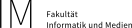
\includegraphics[scale=0.6]{anlagen/bilder/logos/IM-logo}
    \caption{Das Logo von Informatik und Medien }
\end{figure}

\begin{figure}[!t]
    \centering
    \includesvg[width=0.6\columnwidth]{anlagen/bilder/logos/IM-logo.svg}
    \caption{Das Logo von Informatik und Medien }
\end{figure}

Bedenken Sie bei allen Beschriftungen, egal ob Abbildungen, Tabellen oder Quelltexte, dass Sie, sofern diese nicht Ihrer eigenen Schaffenskraft entsprangen,
diese referenzieren. Im Beispiel der Tabelle \ref{tab:Beispieltabelle} sieht man, dass sich der Beschreibungstext direkt an der Tabelle von dem im Tabellenverzeichnis unterscheidet,
genau um den Punkt der Referenz.

\section{Methodik}

Im Methodik-Abschnitt (eine eigene Section) einer Arbeit stellen Sie die Methoden dar, die Sie verwendet haben oder vorhaben zu verwenden, um die Fragestellung zu beantworten. 
In diesem Abschnitt erläutern Sie, welche Methoden umgesetzt wurden (oder auch angedacht), um die Hypothesen zu testen und die Fallstudie durchzuführen. 
Welche Methoden für Ihre Arbeit geeignet sind, ist auch ein wesentlicher Punkt Ihres angestrebten Titels und somit ein zu bewertender Teil dieser Arbeit. 

\underline{Aber \textbf{mindestens} folgende Punkte}\\
Inhalt des ersten Kapitels (im Allgemeinen):
\begin{itemize}
    \item Thematische Einführung, umreißen des Themas \dots wo befinden wir uns?
    \item Herausstellen des Problems und warum es eines ist was gelöst werden sollte.
    \item Herausstellen der tatsächlichen Ziel-/Fragestellung, welche bearbeitet werden wird.
    \item Eine Abgrenzung was diese Arbeit ist und was sie nicht ist.
    \item Stand der Forschung \dots Was existiert bereits? Wie gut passt das auf das Problem?
    \begin{itemize}
        \item Referenzen mittels cite: \cite[S.~111]{jsch2011} \cite[S.~27f]{Tane2014}
    \end{itemize}
    \item Eine abgeleitete Methodik $\rightarrow$ basierend auf der Literatur und Ihrem Wissen: wie haben Sie nun vor Ihr Problem zu lösen? Vllt durch \cite{9429985}?
\end{itemize}


%##########################################################
% Zweites Kapitel
%##########################################################
%!TeX root = ./../MusterAbschlussarbeit.tex

%##########################################################
% Inhalt
%##########################################################

\clearpage
\chapter{Theoretische Grundlagen}
Inhalt des zweiten Kapitels (im Allgemeinen):
\begin{itemize}
    \item Schaffen Sie die theoretischen Grundlagen, welche notwendig sind um Ihre Lösung und deren Mehrwert zu verstehen
    \item Die Tiefe ist an Personen gerichtet, die fachlich zugeordnet sind, aber u.U. kein Fachwissen besitzen:
    \begin{itemize}
        \item Informatiker sind mit dem Programmieren vertraut: Sie brauchen also nicht die Programmiersprache X erklären; jedoch wird nicht jede Person einordnen können was Sie damit machen
    \end{itemize}
    \item Erarbeiten Sie Wissen was im dritten Kapitel als Grundlage für Ihr Konzept dient $\rightarrow$ es ist schwer etwas zu konzipieren, wenn Sie nicht wissen wovon Sie reden
\end{itemize}


%##########################################################
% Drittes Kapitel
%##########################################################
%!TeX root = ./../Bachelorarbeit.tex

%##########################################################
% Inhalt
%##########################################################

\clearpage
\chapter{Konzeption}

Jedes Experiment/oder Softwarekonzeption sollte so detailliert beschrieben werden, dass ein anderer Wissenschaftler die Arbeit durchführen und genau das gleiche Ergebnis erzielen könnte, wie Sie. 
Mit anderen Worten: Ihre Forschung sollte reproduzierbar sein.

Jeder Faktor oder jede Überlegung, die für den Erfolg eines Ihrer Experimente eine wichtige Rolle gespielt hat, muss erwähnt werden.

All diese Punkte schließen natürlich auch ein, dass irgendwie getroffene Abwägungen oder Entscheidungen aufgezeigt und begründet sein müssen. Warum diese Art der Programmierung? Warum dieses Framework?
Alternativen? Am Ende muss für eine lesende Person klar herauskommen, warum Sie Ihre Lösung so konzipiert haben, wie Sie es getan haben und es zudem ein schlüssiger Entscheidungsweg ist. Keine Willkür.

\underline{Aber \textbf{mindestens} folgende Punkte}\\
Inhalt des dritten Kapitels (im Allgemeinen):
\begin{itemize}
    \item Basierend auf dem Fall, dass Sie eine (prototypische) Implementation vornehmen, sollten Sie hier nun diese konzipieren
    \item Wie haben Sie vor die Implementation vorzunehmen? Besonderheiten? Überlegungen? Einflüsse? Probleme?
    \item Gießen Sie Ihre Idee zunächst in ein theoretisches Konstrukt $\rightarrow$ Kapitel Vier ist der Beweis, dass Ihre Überlegungen (nicht) funktionieren.
\end{itemize}


%##########################################################
% Viertes Kapitel
%##########################################################
%!TeX root = ./../MusterAbschlussarbeit.tex

%##########################################################
% Inhalt
%##########################################################

\clearpage
\chapter{Implementation}

Auch wenn der Name des Chapters eher auf eine Art Tagebucheintrag hindeutet, ist der Anteil der Ergebnisdarstellung hier keineswegs zu unterschlagen und unabdingbar.

Unter \enquote{Ergebnisse} sollte eine klare Aussage über die Entdeckungen des Autors gemacht werden, ohne jedoch auf experimentelle Details oder die große Bedeutung der Ergebnisse einzugehen. 
Außerdem müssen die experimentellen Details in diesem Abschnitt auf das beschränkt werden, was für den Leser zum Verständnis der Ergebnisse notwendig ist.

In diesem Kapitel unterscheiden sich maßgeblich zwei Arten von Abschlussarbeiten. In einer Informatik-lastigen Arbeit folgt auf eine Konzeption eine prototypische Implementation,
welche zudem getestet werden muss. Diese Test müssen zum einen ebenfalls \enquote{konzipiert} und begründet werden, sowie in ihren Ergebnissen dargestellt werden.

Eine zweite Art Abschlussarbeit, versteht unter \enquote{Implementation} die eigentliche Durchführung eines Experiments. Die eigentliche Handlungsabfolge (\enquote{1. Stäbchen rein}, etc.) ist dabei 
uninteressant. Daher wird hier gleich auf die Ergebnisse wert gelegt. Hier werden also keine implementationsspezifischen Details dargelegt, sondern gleich die Ergebnisse.

Was beide Ansätz eint, ist eine Interpretation und Kontextualisierung der Ergebnisse. Was sind die Ergebnisse und was \enquote{lesen} Sie daraus ab?
Gern können Sie hier aufgtretene Problem diskutieren, jedoch \textbf{nicht} welchen Wert oder welche Relevanz Ihre Ergebnisse haben.\\


\newpage

Zusammenhängende Ergebnisse werden vorteilhaft in Form von Tabellen (wie in \ref{TabLaufzeiten}) dargestellt.

\begin{table}[h!]
	\begin{center}
        \caption{Laufzeiten in sec, gemessen mit einem Intel xy-8 Ghz Prozessor}\label{TabLaufzeiten}
		\begin{tabular}{|c||c|c|c|}
			\hline 
			& Verfahren X & Verfahren Y & Verfahren Z \\ 
			\hline 
			\hline 
			\hspace{.1cm}
			Problem A & 300 & 340 & 210 \\ 
			\hline 
			\hspace{.1cm}
			Problem B & 730 & 580 & 540 \\ 
			\hline 
			\hspace{.1cm}
			Problem C & 610 & 420 & 440 \\ 
			\hline 
			\hspace{.1cm}
			Problem D & 895 & 790 & 520 \\ 
			\hline 
		\end{tabular} 
	\end{center}
\end{table}


Funktionale Zusammenhänge hingegen lassen sich in Form von Diagrammen oder Grafiken (Siehe \ref{fig:Abbildung1}) darstellen.


\begin{figure}[!htb]
	\centering
	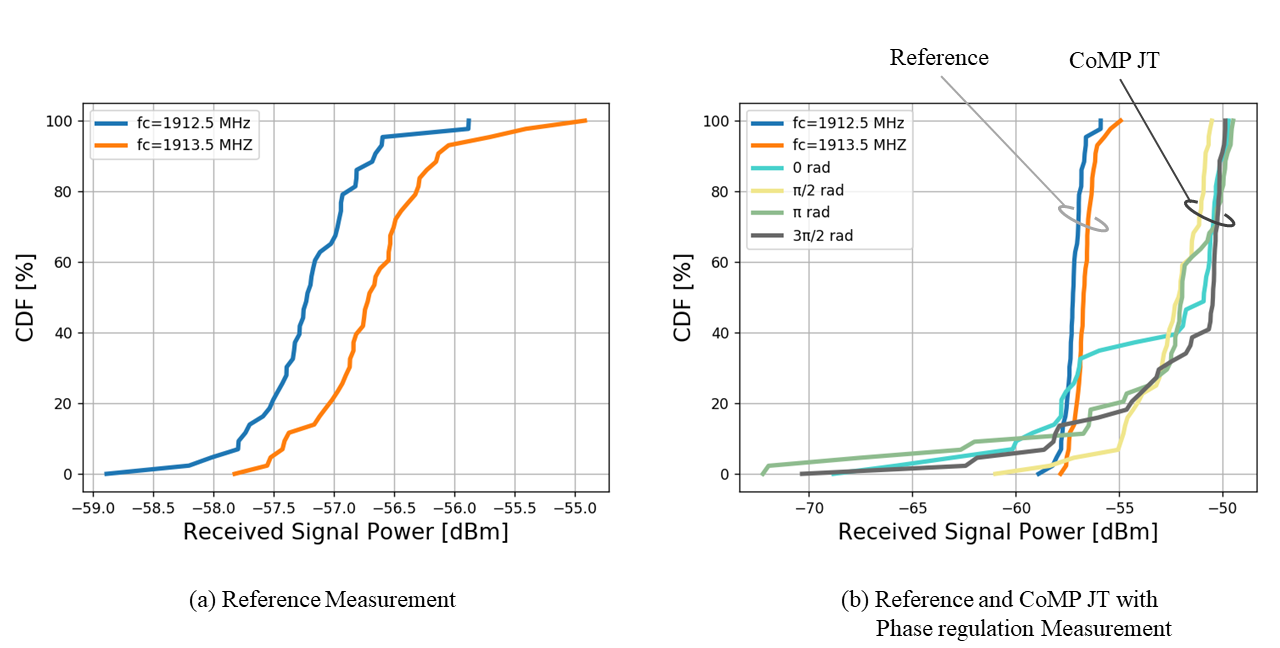
\includegraphics[width=1\textwidth]{Bilder/Abbildung1}
	\caption{Statistical analysis of the received power}
	\label{fig:Abbildung1}
\end{figure}

Ein guter Ergebnisteil erfordert Literaturzitate (vielleicht auch gar keine) und die Bekanntgabe des Ergebnisses sollte von einer Interpretation und Diskussion begleitet werden. 


\newpage

\underline{Aber \textbf{mindestens} folgende Punkte}\\
Inhalt des vierten Kapitels (im Allgemeinen):
\begin{itemize}
    \item Setzen Sie nun den Plan aus dem dritten Kapitel wenigstens prototypisch um
    \item Ziel ist es Ihre Überlegungen und Darlegungen zu beweisen
    \item Diskutieren von Problemen
    \item Zusätzlich zu der Umsetzung bedarf es (von Ihnen zu definierender) Tests, um die Funktionalität zu beweisen
    \begin{itemize}
        \item Laufzeittests, Lasttests, etc.
        \item Produzieren Sie Ergebnisse um zu zeigen, dass Ihr Ansatz funktioniert und besser/schlechter ist
        \item \glqq schlechter\grqq{} sein, bedeutet nicht, dass Ihre Arbeit schlecht ist! Am Ende zählt Ihr Ansatz und die Idee
    \end{itemize}
\end{itemize}


%##########################################################
% Fünftes Kapitel
%##########################################################
%!TeX root = ./../Bachelorarbeit.tex

%##########################################################
% Inhalt
%##########################################################

\clearpage
\chapter{Auswertung und Ausblick}

Dieser Abschnitt stellt den Schlusspunkt der Arbeit dar. In diesem Abschnitt (und im Diskussionteil) erwartet der Leser, 
dass er Antworten auf die in der Einleitung formulierten Fragestellungen findet und sich vergewissert, 
dass diese wirksam verteidigt wurden und mit der von Ihnen formulierten \enquote{These} übereinstimmen.

Die Hauptziele der Diskussion bestehen darin, eine Analyse Ihrer gesammelten Ergebnisse zu präsentieren, 
Ihre Ergebnisse angemessen darzustellen und eine Einschätzung der Bedeutsamkeit Ihrer Arbeit zu geben. Beachten Sie hier,
den Unterschied zur Diskussion im vorherigen Kapitel. Diskutieren Sie hier vor allem den Wert und die Bedeutung Ihrer Ergebnisse, auf Basis der 
Interpretationen aus dem vorherigen Kapitel. Beziehen Sie sich gern auch auf Ihr beschriebenes Problem und Ihr Ziel.

Jede wichtige Schlussfolgerung, die Sie im \enquote{Ergebnisteil} gezogen haben, 
muss hier erneut behandelt werden. Eine gewisse Anzahl von Wiederholungen ist unvermeidlich. Darüberhinaus, 
die Ergebnisse anderer Forschungsarbeiten, müssen mit eindeutigen Verweisen auf auffindbare Literaturquellen versehen sein.

Der Fazit-Teil kann als eine kurze Zusammenfassung Ihrer Diskussion betrachtet werden. 
Der Leser muss sich hier schnell einen Überblick über den Inhalt und die Bedeutung der Arbeit als Ganzes verschaffen.

Dieser Abschnitt soll einen Überblick präsentieren und dient dazu, dem Hauptteil Ihrer Arbeit den letzten Schliff zu geben. 
Die Schlussfolgerung kann auch Hinweise auf ein mögliches zukünftiges Werk enthalten.

\underline{Aber \textbf{mindestens} folgende Punkte}\\
Inhalt des fünften Kapitels (im Allgemeinen):
\begin{itemize}
    \item Reflektieren Sie hier nun die Ergebnisse der Tests aus dem letzten Kapitel
    \item Ordnen Sie diese in den Gesamtkontext ein... gut/schlecht? Was kann man verbessern/anders machen? Schätzen Sie auch ab was Veränderungen bringen könnten.
    \item Was wurde durch die Ergebnisse gezeigt? Geben Sie eine bewertende (selbstkritische) Aussage ab zu Ihrem Schaffen
    \item Geben Sie einen Ausblick was nun folgen sollte/könnte.
\end{itemize}


%##########################################################
% Literatur
%##########################################################
%!TeX root = ./../Bachelorarbeit.tex

%##########################################################
% Inhalt
%##########################################################
\printbibliography[title={Literaturverzeichnis}, heading=bibintoc]


%##########################################################
% Anhang - nicht verwendete Anhangsseiten bitte kommentieren
%##########################################################
\appendix
\pagenumbering{Roman}
\setcounter{page}{1}

%!TeX root = ./../Bachelorarbeit.tex

%##########################################################
% Inhalt
%##########################################################
\clearpage
\chapter{Anhang -\ Abbildungen}

Grundsätzlich gehören Tabellen und Abbildungen in den Hauptteil der Arbeit.
Hat man aber sehr viele oder auch lange Tabellen, die den Lesefluss im Hauptteil
stören würden, dann können diese in einen separaten Anhang aufgenommen werden.
Wichtig ist in jedem Fall, dass zwischen Hauptteil und Material im Anhang durch
geeignete Verweise eine Beziehung hergestellt wird.

%!TeX root = ./../Bachelorarbeit.tex

%##########################################################
% Inhalt
%##########################################################
\clearpage
\chapter{Anhang -\ Tabellen}

%!TeX root = ./../Bachelorarbeit.tex

%##########################################################
% Inhalt
%##########################################################
\clearpage
\chapter{Anhang - Quelltexte}
Auch längere Quelltexte gehören nicht in den Hauptteil,
sondern entweder in den Anhang oder bei großem Umfang nur auf
ein erreichbares Repository (Gitlab o.ä.).
Wünscht man Algorithmen im Hauptteil zu erklären, dann kann dies durch Pseudocode erfolgen.


% ***********************************************
\end{document}
% ***********************************************
